
%\subsection{Redes Neuronales}

\begin{frame}{Aprendizaje Máquina (Machine Learning)}

Es una disciplina de la IA que por medio de \textbf{algoritmos y datos}, permite a las computadoras imitar la forma en la que los humanos aprenden, mejorando su precisión de manera gradual
\begin{columns}
\begin{column}{0.48\textwidth}
\begin{itemize}
\item Aprendizaje Supervisado: se requiere tener conocimiento previo de etiquetas asignadas a los datos para poder generar el modelo
\item Aprendizaje No supervisado: intentan descubrir patrones ocultos o agrupamientos de datos sin requerir de intervención humana
\end{itemize}
\end{column}
\begin{column}{0.52\textwidth}  
    \begin{center}
     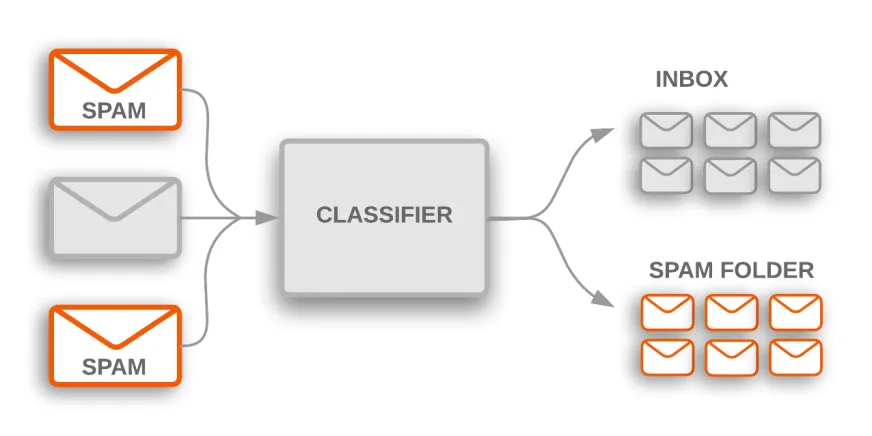
\includegraphics[width=\textwidth]{00_IntroMachineLearning/figs/Classifier}
     \end{center}
\end{column}
\end{columns}


\end{frame}

\begin{frame}{Aprendizaje Máquina vs Aprendizaje Profundo}
%\Huge

	%\begin{block}{Aprendizaje Máquina} 
		\begin{columns}
		\begin{column}{0.57\textwidth}
		\begin{block}{Aprendizaje Máquina} 
		\begin{itemize}
		\item Se requiere de una fase de \textbf{extracción de características} de los datos de entrada
		\item Existen múltiples algoritmos, uno de los más representativos son las Redes Neuronales
		\end{itemize}
		\end{block} 
        \begin{block}{Aprendizaje Profundo} 
		\begin{itemize}
		\item La fase de \textbf{extracción de características} no es necesaria
        \item Principalmente basadas en redes neuronales
%		\item Una generación de algoritmos que permiten resolver tareas.
		%\item Las computadoras intentan resolver tareas que solo son posibles mediante inteligencia humana
		%\item Es una rama muy amplia que cubre muchos aspectos de la vida cotidiana.
		\end{itemize}
		\end{block} 

		\end{column}
		\begin{column}{0.37\textwidth}  
			\begin{center}
			 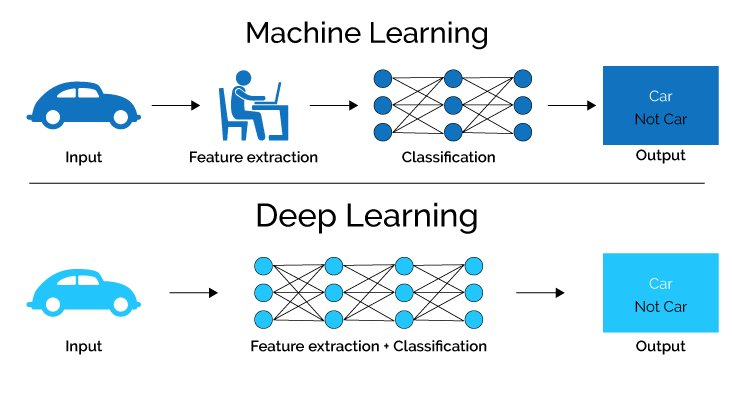
\includegraphics[width=\textwidth]{Figs/MachineLearningVsDeepLearning}
			 %\includegraphics[width=\textwidth]{WordReading2}
			 \end{center}
		\end{column}
	\end{columns}
	%\end{block} 
\end{frame}

